\documentclass[a4paper,12pt]{article}
\usepackage[center]{caption}
\usepackage[pdftex]{graphicx}
\usepackage[pdftex]{hyperref}
\usepackage{amsmath}
\usepackage{subfig}
\usepackage{listings}
\usepackage{latexsym}
\usepackage{pdflscape}
\usepackage{fancyhdr}

% Setup fancy headings - copied from lshort
\pagestyle{fancy}
% with this we ensure that the chapter and section
% headings are in lowercase.
\renewcommand{\sectionmark}[1]{%
        \markright{\thesection\ #1}}
\fancyhf{} % delete current header and footer
\fancyhead[LE,RO]{\bfseries\thepage}
\fancyhead[LO]{\bfseries\rightmark}
\fancyhead[RE]{\bfseries\leftmark}
\renewcommand{\headrulewidth}{0.5pt}
\renewcommand{\footrulewidth}{0pt}
\addtolength{\headheight}{0.5pt} % space for the rule
\fancypagestyle{plain}{%
   \fancyhead{} % get rid of headers on plain pages
   \renewcommand{\headrulewidth}{0pt} % and the line
}

\newcommand{\graphwidth}{5.8cm}

% From wikipedia
\DeclareMathOperator*{\argmax}{arg\,max}
\DeclareMathOperator*{\argmin}{arg\,min}

\lstset{breaklines=true,basicstyle=\small,tabsize=3,numbers=left,numberstyle=\tiny,numbersep=5pt,emptylines=1}

\lstdefinelanguage{Cg}
	{morekeywords={const,float,float2,float3,float4,float4x4,uniform,in,out,sampler3D,int,void,TEXCOORD0,COLOR0,TEXUNIT0,TEXUNIT1,cos,sin,return,for},
	sensitive=true,
	morecomment=[l]{//},
	}

\title{3D Model Fitting and its Use in Gait Recognition - a Summary}
\author{David Sansome}

\begin{document}
\bibliographystyle{plain}

\maketitle

\begin{abstract}
	Gait recognition is an area of biometrics that focuses on identifying people by the way they walk.
	Gait recognition has the advantage over other biometrics, such as fingerprint or iris recognition, in that it can be used from a distance and without the subject's knowledge.
	
	Previous attempts to tackle gait recognition through model-fitting have used 2D videos of subjects captured by a single camera.
	This is the first work that uses a 3D representation of a person, constructed by combining images from multiple cameras.
	
	The final algorithm was able to correctly recognise 90\% of the test subjects.
\end{abstract}

\tableofcontents


\newpage
\section{Overview}

\begin{figure}[b]
	\centering
	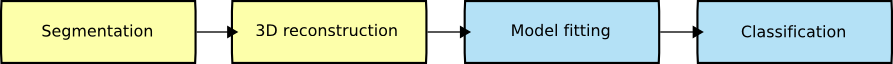
\includegraphics[width=12cm]{../report/overview.png}
	\caption{The main stages in gait recognition.
		Those coloured blue are the ones tackled in this project.}
	\label{OverviewBoxes}
\end{figure}

The four main stages in gait recognition are shown in Figure \ref{OverviewBoxes}.
Our data was obtained from the University of Southampton Gait Tunnel -
a walkway in which the walls are lined with a number of cameras to capture images of the subject's face and ears, as well as the motion of his legs and body as he walks.
This data takes the form of several colour videos, so the first step is to isolate the walking figure by segmentation and background subtraction.
Next all these videos are combined together into one three-dimensional video in a process known as 3D reconstruction.

Now we have a single 3D video, the next stage is to extract information that we can use to identify the subject.
We do this by attempting to fit a model to the subject's legs.
This will give us a set of parameters that describe certain properties of the legs in each frame - eg. their angle made with the hip.
By looking at how these parameters change over time, we can form a signature that uniquely describes the subject.
Comparing the signature to a database of other signatures allows us to classify the subject and determine his identity.

This project focuses on only the final two stages - the model fitting and classification.
The data we use for testing has already undergone 3D reconstruction and is in the form of a series of frames containing voxelized images of the subject.


\newpage
\section{Implementation}

\subsection{A Model for Human Gait}

\begin{figure}[hb]
	\centering
	\subfloat[Side view]{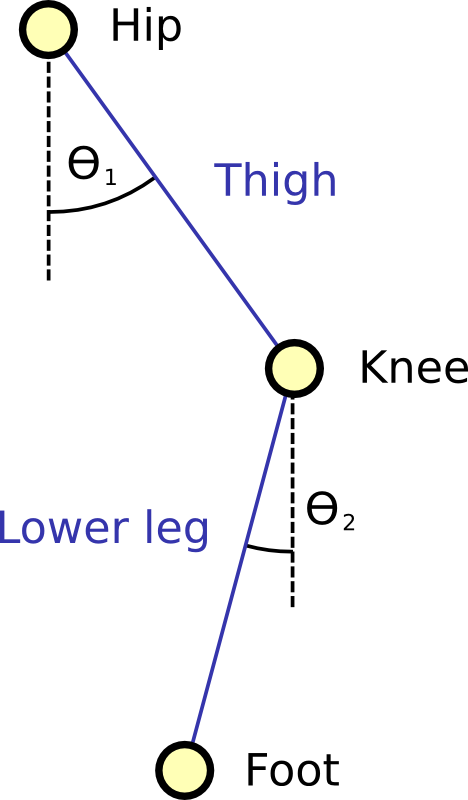
\includegraphics[height=6cm]{../report/model1.png}}
	\qquad
	\subfloat[Front view]{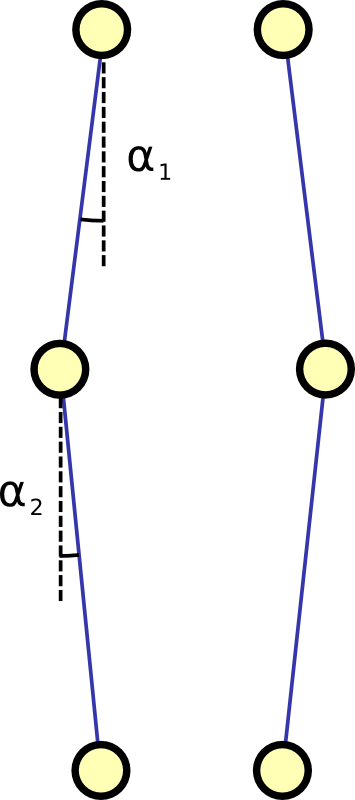
\includegraphics[height=6cm]{../report/model2.png}}
	\caption{Our model for the human leg.}
	\label{ModelImages}
\end{figure}

The very first stage is to define exactly how the human leg can move and what parameters we can extract from it.

Figure \ref{ModelImages} shows our model for the human leg.
At the top of the model is the hip which we take to be fixed half-way between the ground and the subject's head.
Connected to this is the thigh which is free to pivot about the hip in two axes.
The angles the thigh makes with the vertical are denoted by $\theta$ and $\alpha$.
$\theta$ is the angle in the direction of travel, and $\alpha$ is the angle perpendicular to the direction of travel.


\subsection{Fitting the Model to a Video Frame}

In order to determine how well a particular orientation of the model fits to one frame in the video, we need to create a 3D filter that we can match to the voxel data.
The first attempt at this involved creating a 20x20x20 filter in which each of the voxels held a value $i \in \{0 \cdots 1\}$.
The energy of this filter at a particular orientation was obtained by simply multiplying each filter voxel with the corresponding voxel in the sample data and summing the results.

This first attempt was inadequate as it relied only on matching filled voxels.
It suffered from the problem that the filter tended to fit better when aligned diagonally across both legs - in the position where it can match the greatest number of voxels.
To correct this problem we created a new filter that was more intelligent about the types of voxels it matched.

\begin{figure}[p]
	\centering
	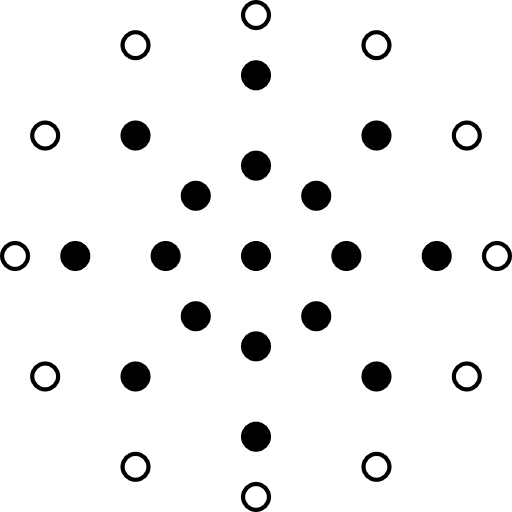
\includegraphics[width=4cm]{../interim/improvedfilter.png}
	\caption{A cross section through the cross-correlation filter.
		Black circles represent filled voxels, and white circles represent edge voxels.}
	\label{ImprovedFilterCross}
\end{figure}

\begin{figure}[p]
	\centering
	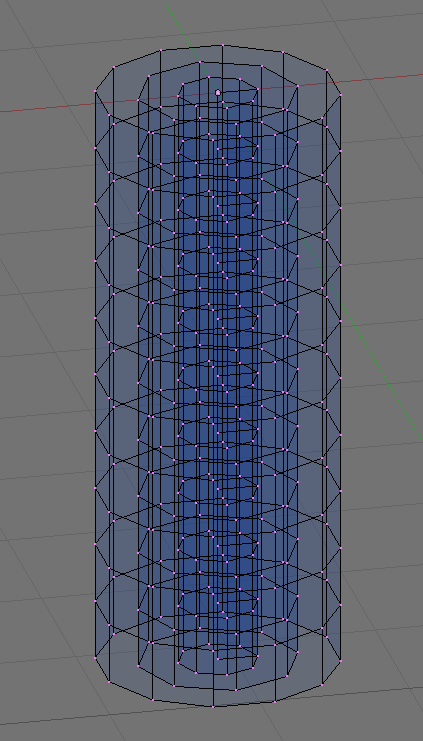
\includegraphics[width=5cm]{../report/thighmodel.png}
	\caption{The cross-correlation filter rendered in the Blender application \cite{Blender}.
		Although not shown in this image, the outer points in the mesh are coloured white to indicate that they should
		match only edge voxels.}
	\label{ImprovedFilter}
\end{figure}

The improved filter shown in Figures \ref{ImprovedFilterCross} and \ref{ImprovedFilter} is a mesh that consists of two types of nodes - those that seek edge voxels and those that seek filled voxels.
This is a similar approach to the one taken by Nixon et al.\ in \cite{GaitBook}.

\clearpage
To fit this mesh to the voxel data we use a least squares linear regression method, like that used by Zhihui et al. \cite{LinearModelFitting}.
Figure \ref{FittingImages} shows a two-dimensional example to demonstrate this least squares fitting, however three dimensional fitting works in exactly the same way.
The goal is to fit a mesh (shown as black dashed lines) to voxel data in the shape of a leg (shown as a filled green rectangle).
The mesh contains a number of nodes which are shown in the diagrams as filled circles.
Yellow circles are trying to match edge voxels, and blue circles are trying to match filled non-edge voxels.

\begin{figure}[bt]
	\centering
	\subfloat[High energy fitting]{\label{FittingImageHigh}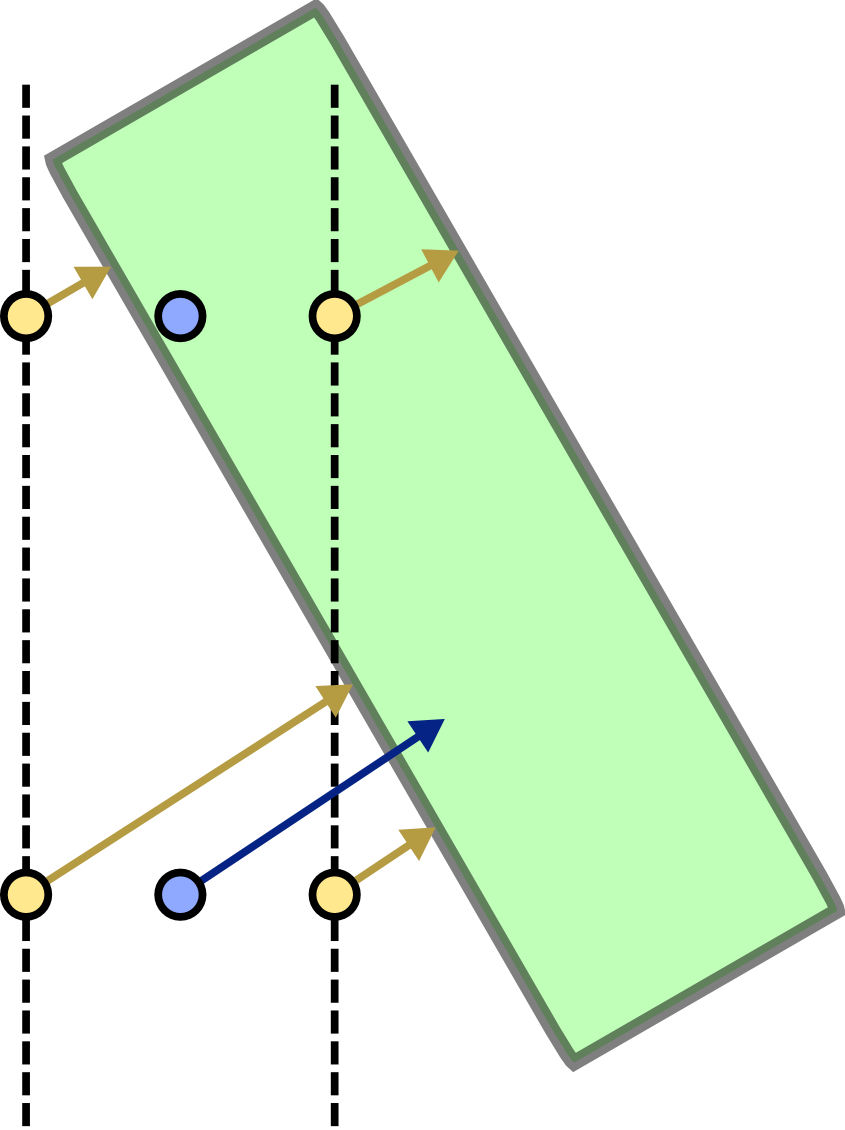
\includegraphics[height=6cm]{../report/fitting1.png}}
	\qquad
	\subfloat[Low energy fitting]{\label{FittingImageLow}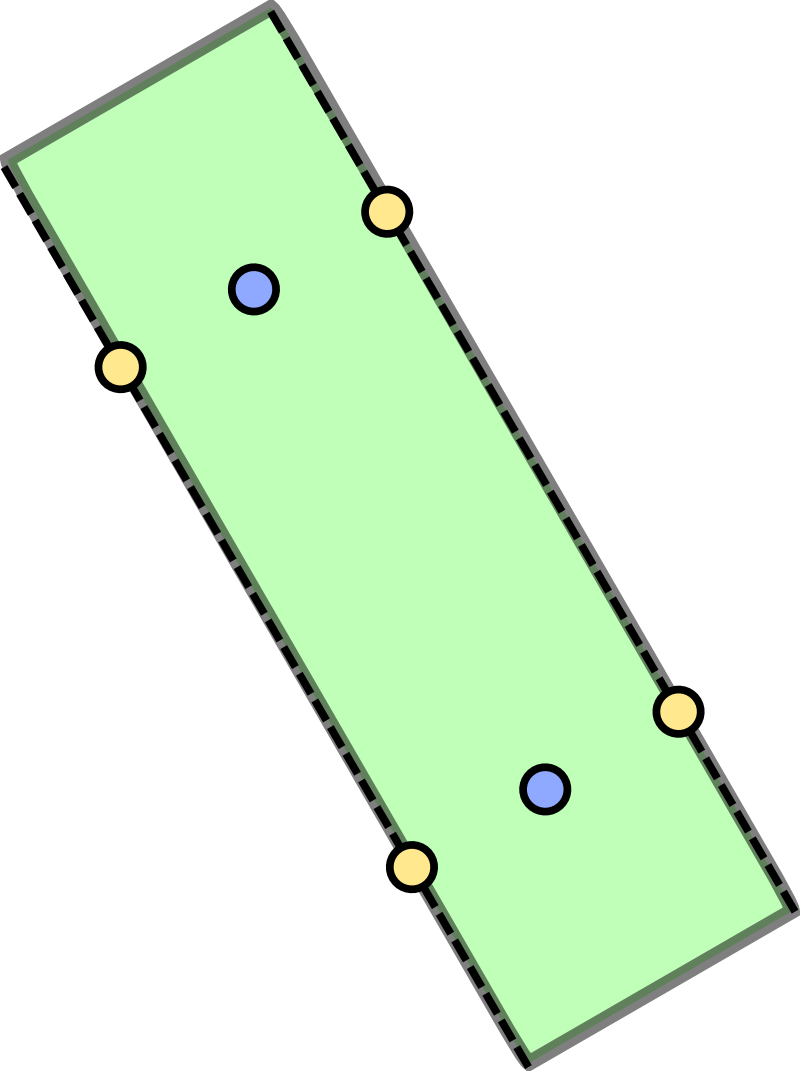
\includegraphics[height=6cm]{../report/fitting2.png}}
	\caption{Potential fittings of our mesh filter.
		The filled green rectangle represents the voxels of a subject's thigh,
		and the coloured circles show a few of the nodes in the mesh.}
	\label{FittingImages}
\end{figure}

An algorithm iterates over the six nodes in the mesh, and for each one searches for the nearest suitable voxel (for the yellow nodes, only edge voxels are suitable).
The first potential fitting, Figure \ref{FittingImageHigh}, has the mesh orientated straight down ($\theta = 0$) and only one of the nodes - the blue one at the top - lies directly on top of a suitable voxel.
The sum of the squared distances between each of the nodes and its closest suitable voxel is taken, and this is used as the overall ``energy'' of that orientation.
Figure \ref{FittingImageHigh} has a high energy as the distances between the nodes and their voxels is very large.
Figure \ref{FittingImageLow} has an energy of $0$, as each node lies directly on top of a suitable voxel.

We can store the energies at each orientation of the model and use them to plot a graph.
Figure \ref{EnergyPlot} shows the energy for the left thigh in one frame of a sequence.

\begin{figure}[bt]
	\centering
	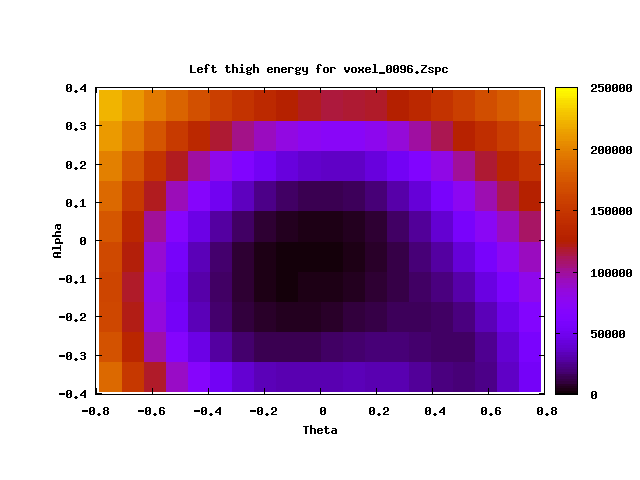
\includegraphics[width=\textwidth]{../report/problems/set81frame96-fixed-leftthigh.png}
	\caption{Energy plot of Frame 96 from Sample 81.
		Darker colours represent lower energies.}
	\label{EnergyPlot}
\end{figure}

We can see from the plot that there is a minimum around the centre - where $(\alpha_1, \theta_1) = (0, 0)$ and the thigh is pointing straight down.

\bigskip
An exhaustive search such as this one takes a very long time to iterate over the entire parameter space and produce a result.
Several tricks were employed that reduced execution time from several hours per frame to a couple of seconds.

MapReduce \cite{MapReduce} was used to split the problem into a number of small tasks and distribute them between processors in a multi-core system.
On the dual-core development machine this brought about a speed increase of almost 2x, but the technique would also scale well to larger clusters.

A \emph{map} function is defined which takes a piece of input data (the parameters) and maps them to a result (the energy of the model with those parameters).
The \emph{reduce} function then gathers up several of these results and reduces them down into one.
Our implementation eliminates the one with the highest energy and keeps the one with the lowest energy.
In this way all the intermediate results from the map functions get reduced into one final result which contains the parameters that fit best.
Figure \ref{MapReduceDiagram} shows how this idea works.

\begin{figure}[bt]
	\centering
	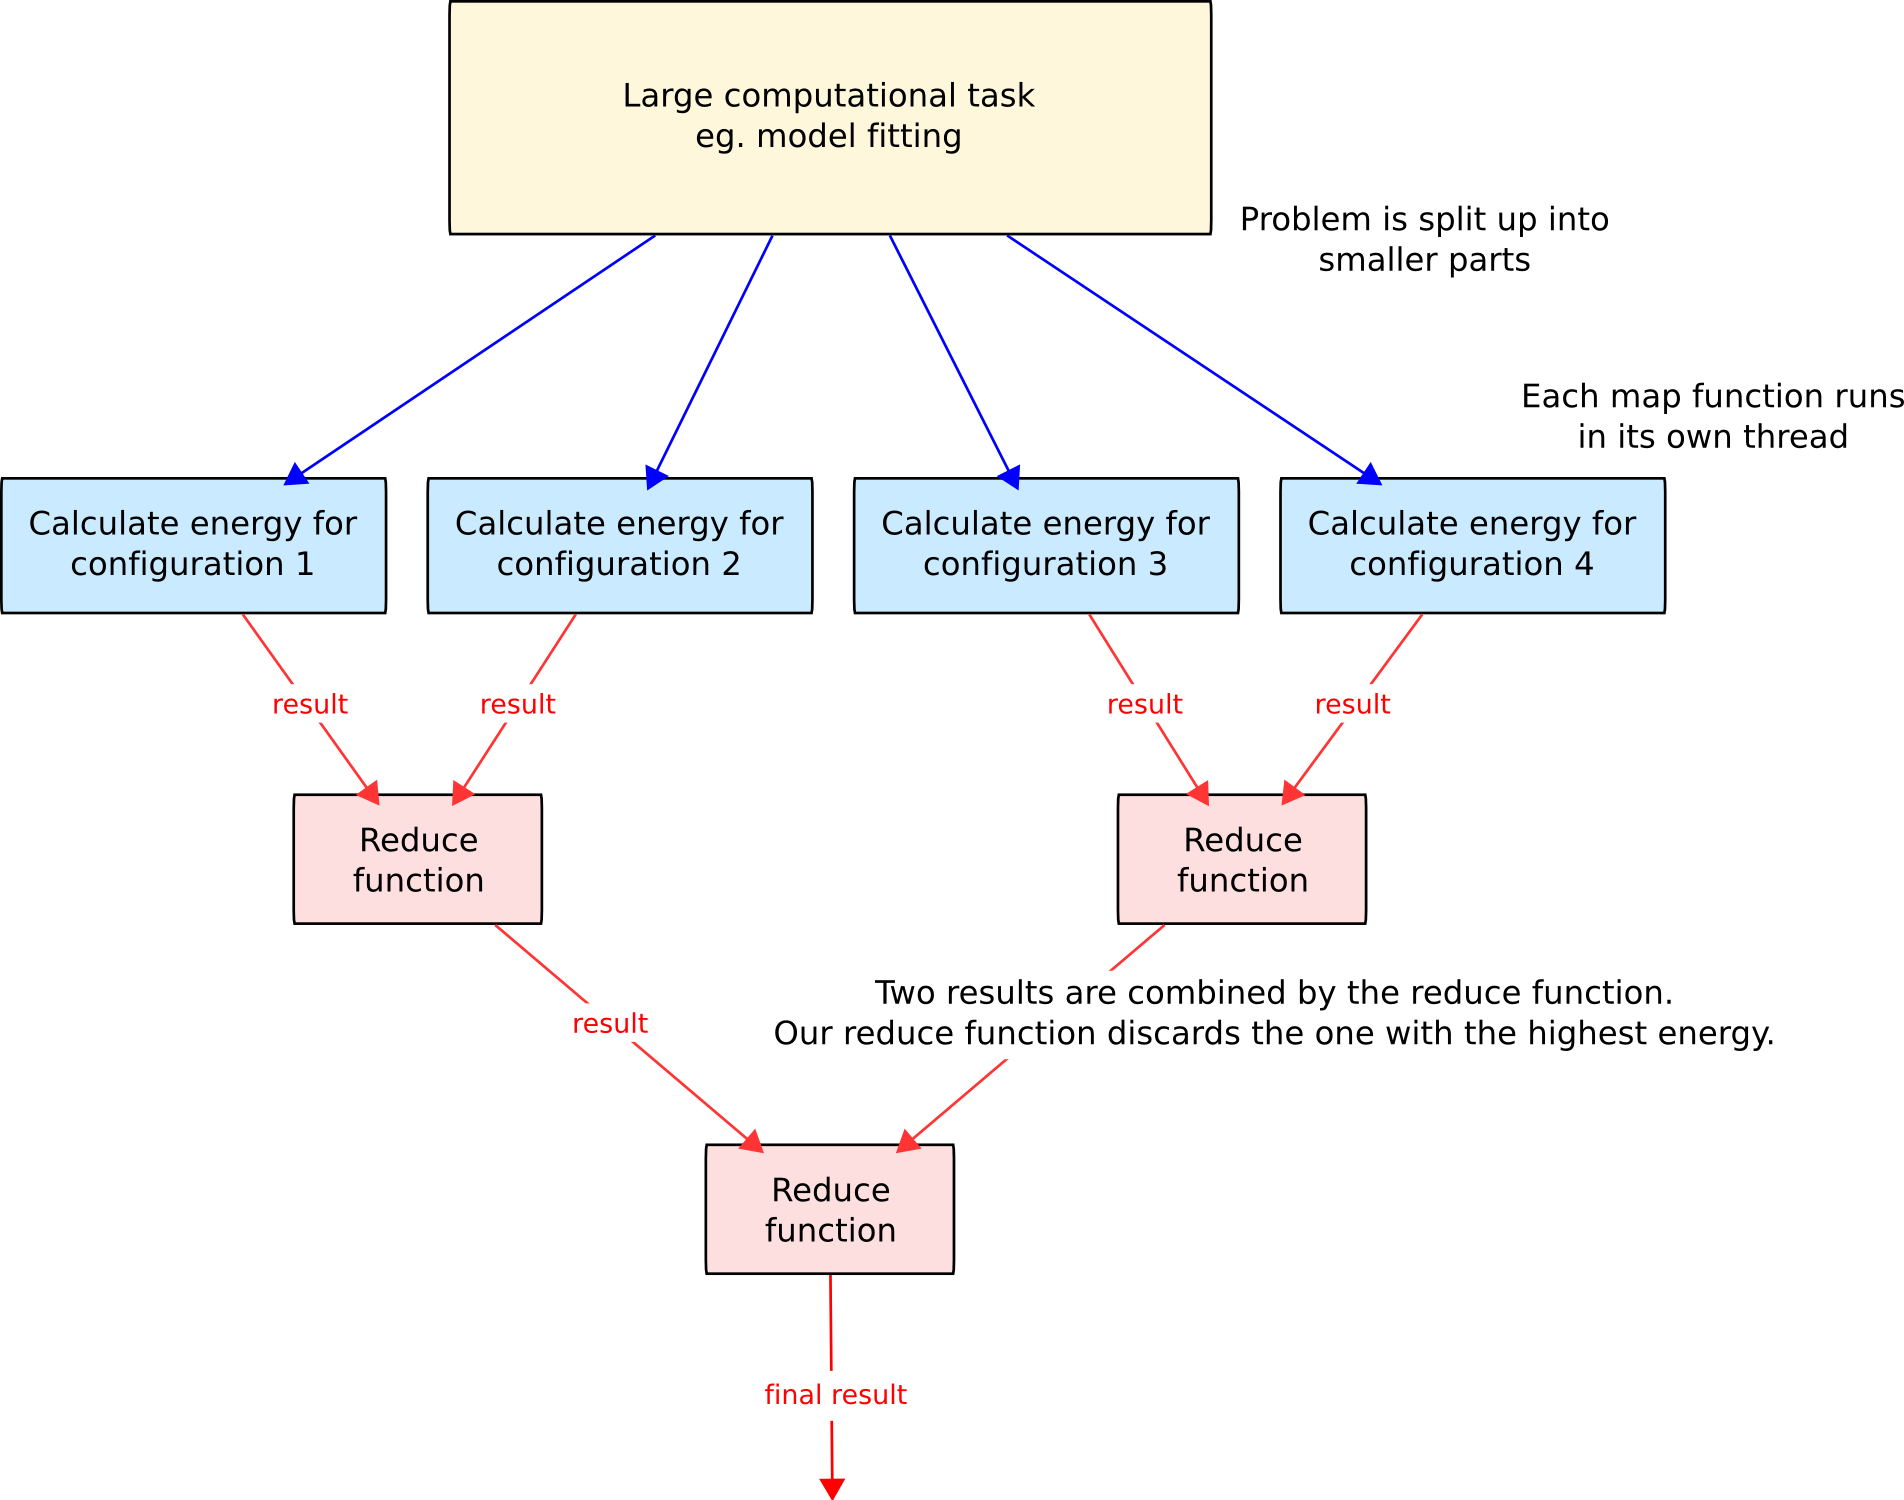
\includegraphics[width=\textwidth]{../report/mapreduce.png}
	\caption{A diagram showing how MapReduce may be used to parallelise and speed up modelfitting.}
	\label{MapReduceDiagram}
\end{figure}

\bigskip
The most expensive functions in the modelfitting algorithm are those which search for nearby voxels of a given type.
These lookups are repeated over and over again as the algorithm ``moves'' the mesh around the voxel-space.
In fact, with a 41x41x11x11 parameter space and 319 points in the mesh, almost 65 million ``how far is the nearest voxel'' queries are performed.
In the worst case, where the mesh is nowhere near the actual limb it is searching for, this could lead to a total of 86,361 million calls to the Voxel\_Space's get() function.

A caching system was implemented that allows the algorithm to store the results of these lookups, so that the next time that value is needed it can be pulled straight from the cache instead of being calculated again from scratch.
Introducing this cache reduced execution time of a typical frame from over two hours to under two minutes.

\bigskip
The initial algorithm searched over the parameter space at a fixed resolution.
In the majority of energy plots there is only one minimum, so we can reduce processing time by sampling the parameter space more intelligently.

If we run one search over the whole parameter space at a low resolution, we can then run a second high resolution search centred on the minimum found by the first search.
This will save us sampling the energy function in thousands of places where there can't possibly be a minimum.
Figure \ref{MultiResImages} demonstrates the principle behind this idea - the second pass is centred on the minimum found in the first pass.

\begin{figure}[bt]
	\centering
	\subfloat[First pass]{\label{MultiResImage1}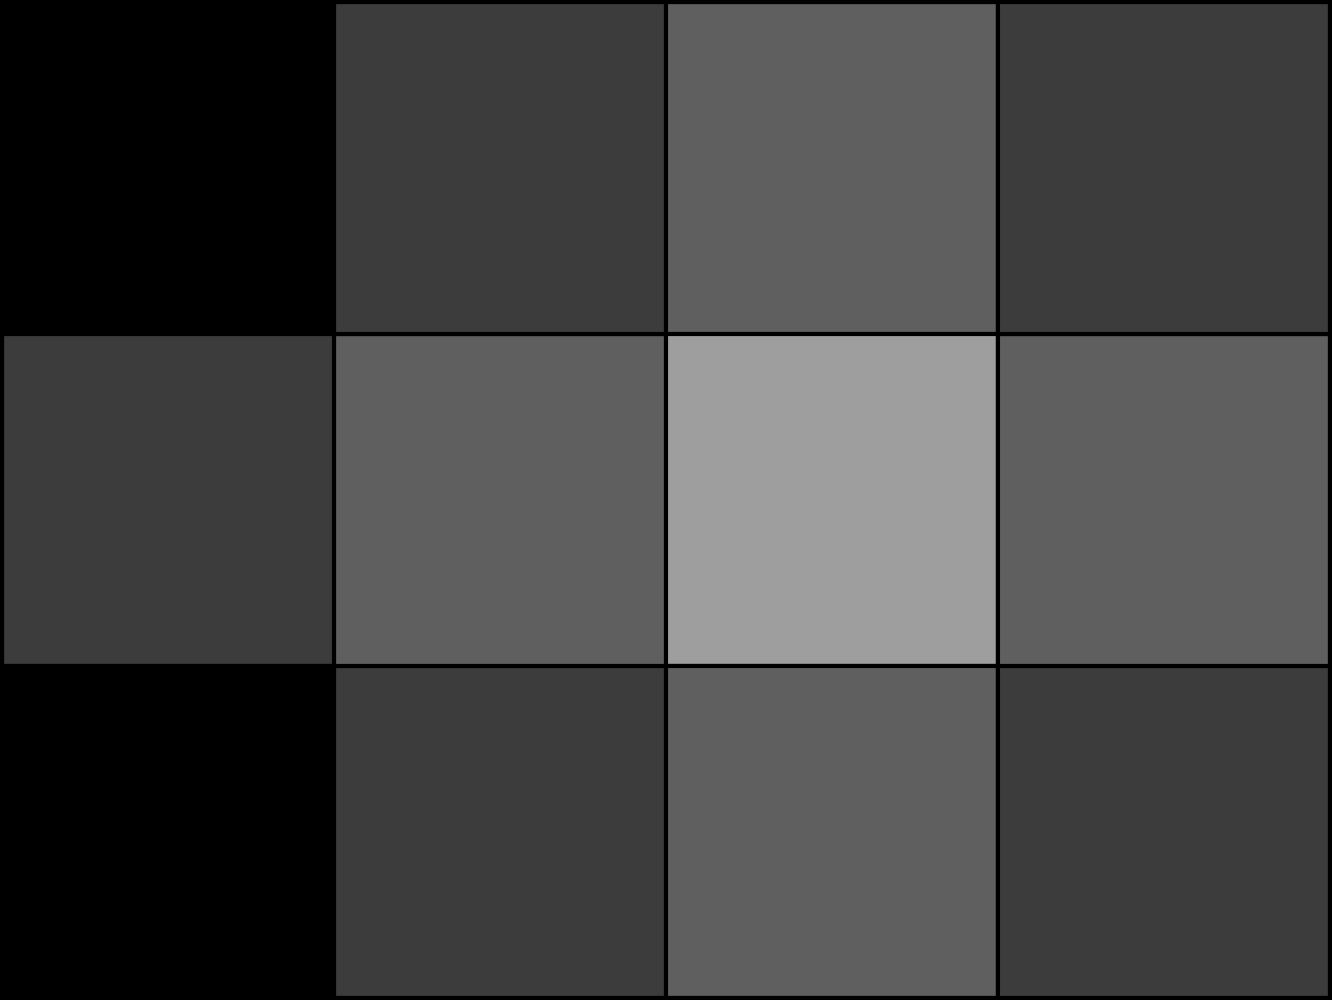
\includegraphics[width=5cm]{../report/multires1.png}}
	\qquad
	\subfloat[Second pass]{\label{MultiResImage2}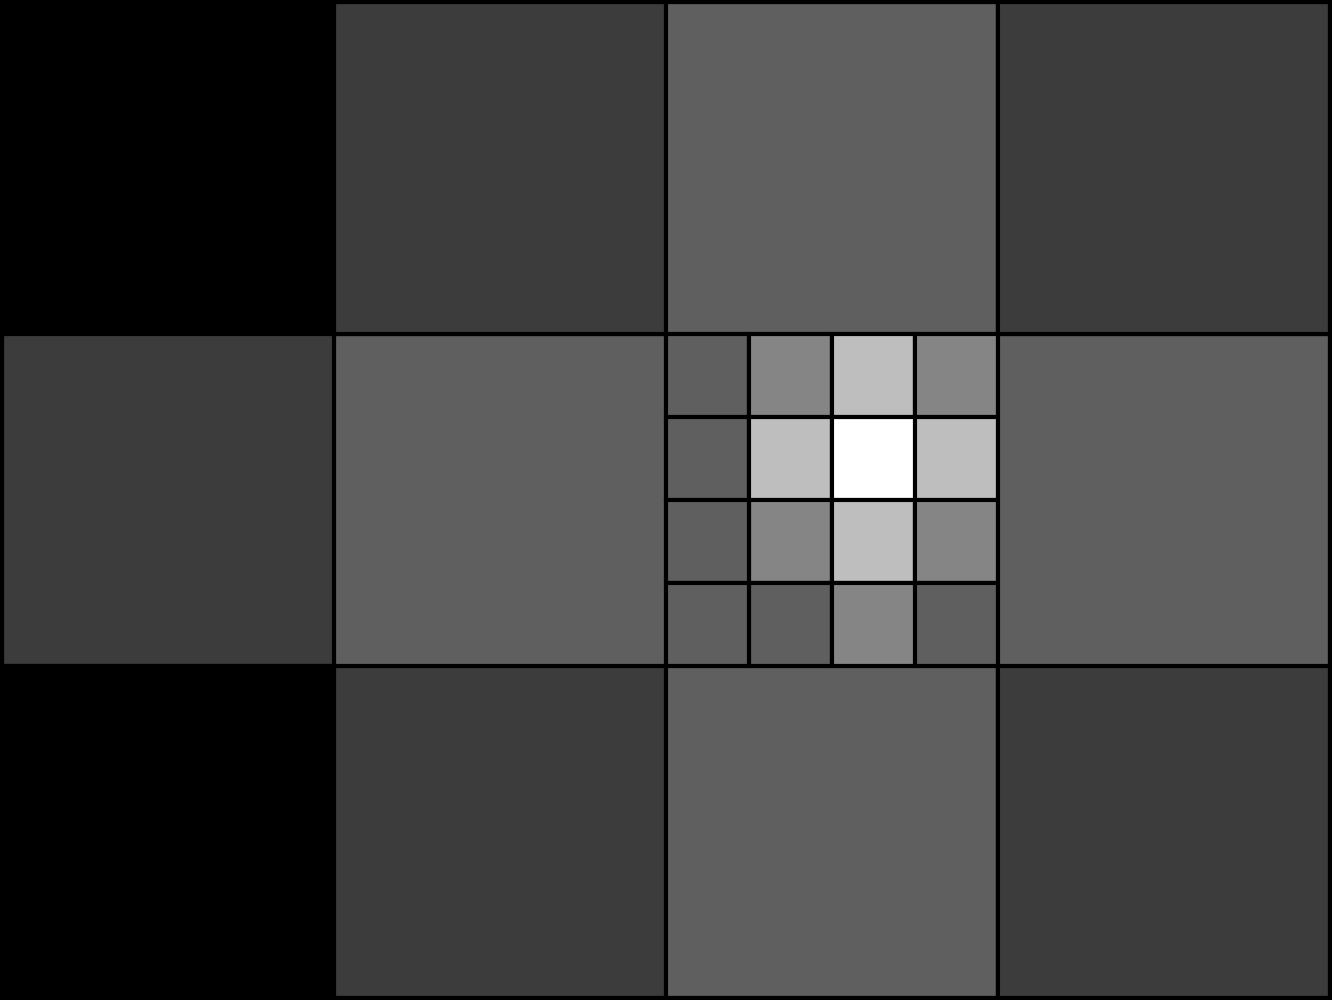
\includegraphics[width=5cm]{../report/multires2.png}}
	\caption{The multiresolution search approach uses two passes - the first is at a low resolution over a large area,
		and the second is at a high resolution over a small area.}
	\label{MultiResImages}
\end{figure}

Implementing multi-resolution search reduced execution time by more than a factor of four.


\subsection{Producing a Gait Signature}

After every frame in a sample has been through the modelfitting process, we can analyse the sequence as a whole
and produce a series of numbers (a \emph{signature}) which describe the subject's gait.
If we are successful, this signature will be unique to each subject and can be used as the basis for classifying any new samples.

\begin{figure}[p]
	\centering
	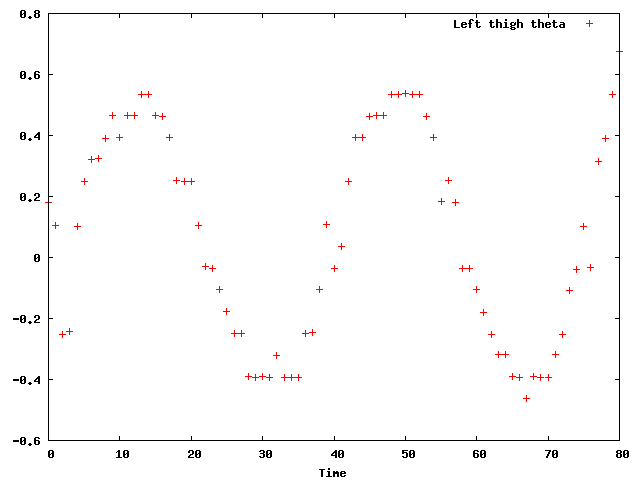
\includegraphics[width=\textwidth]{../report/curvefitting.png}
	\caption{The change in $\theta_1$ over time for Sample 81.}
	\label{CurveFitting1}
\end{figure}

Figure \ref{CurveFitting1} shows how a subject's left thigh moves over time.
We can intuitively see that this is correct - as we walk our legs swing backwards and forwards in a sinusoidal fashion.
From the graph it can be seen that the forwards motion of the leg is slightly faster (or steeper) than the backwards motion of the leg.
It is subtle features like these that can be used to uniquely identify a subject.

\begin{figure}[p]
	\centering
	\subfloat[Magnitude]{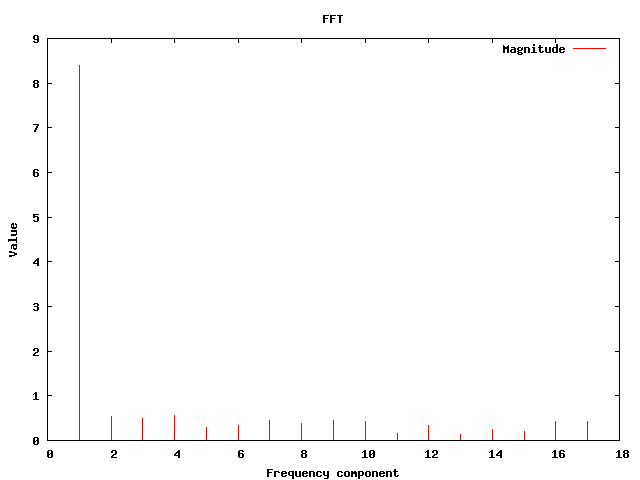
\includegraphics[width=6cm]{../report/dft-leftthightheta-magnitude.png}}
	\quad
	\subfloat[Phase]{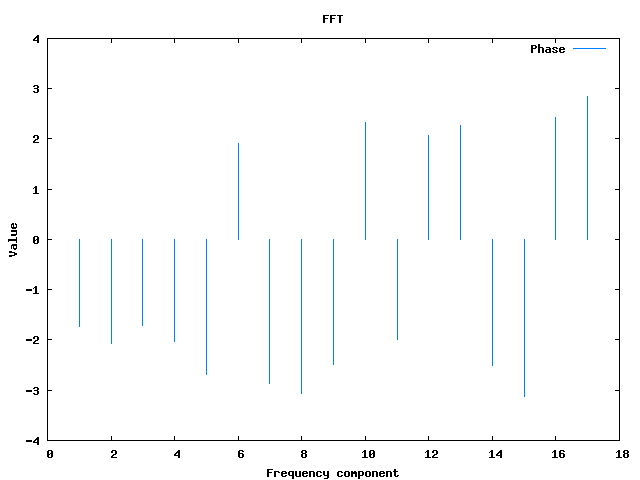
\includegraphics[width=6cm]{../report/dft-leftthightheta-phase.png}}
	\caption{Results of taking the DFT of $\theta_1$ from one gait cycle of Sample 81.}
	\label{FFTResults}
\end{figure}

To extract these features from the graph we take the \emph{discrete Fourier transform} (DFT).
Figure \ref{FFTResults} shows the phase and magnitude plots of one cycle of one subject's gait.
The real and imaginary components of the Fourier transform are used to build a feature vector, or \emph{signature}, for a subject.

BenAbdelkader et al.\ \cite{StrideCadence} showed how static parameters - height, torso length, leg length and step length - can also be used to classify subjects.
Including the body height in our feature vector greatly improved the classification rate.

\subsection{Classifying an Individual}

To correctly classify a new sample, we need some way of comparing it to the other samples already in the database.
The k-nearest neighbour algorithm with $k=1$ was chosen as it is straightforward to implement while providing good results.

A distance function $d(a,b)$ was created to compare and evaluate the difference between two samples $a$ and $b$.
Several implementations of this distance functions were created and tested against the dataset to see which one provided the best results.

Those tested include:

\begin{enumerate}
	\item Straightforward comparison of magnitude components.
	\item Magnitude-weighted phase.
	\item Euclidean distance in the complex plane.
	\item Polar distance.
\end{enumerate}

These distance functions were each tested before and after mean normalisation, and exclusion of the first frequency component.


\newpage
\section{Results}

A manual fitting was produced for selected samples to provide a means of evaluating the error of the modelfitting algorithm.
Each frame was examined in the modelfitting application, and the parameters of the model tweaked to visually fit the model to the image of the subject.

The error between the manually entered result $m_t$ and the automatically determined result $a_t$ for a sample with $N$ frames was calculated as follows:

\begin{equation}
	E = \frac{1}{N} \sum_{t=1}^N \left| a_t - m_t \right|
\end{equation}

The values in the table below represent the average error per frame as a percentage of the possible range for $\theta$ ($\pm \frac{\pi}{4}$).

\begin{table}[thb]
	\centering
	\begin{tabular}{l|cc|cc|cc}
		& \multicolumn{2}{|c|}{Low fixed res} & \multicolumn{2}{|c|}{High fixed res} & \multicolumn{2}{|c}{Multi-resolution} \\
		& 81 & 96 & 81 & 96 & 81 & 96 \\
		\hline
		Left thigh & 2.94\% & 1.83\% & 3.18\% & 1.97\% & 3.01\% & 1.48\% \\
		Right thigh & 2.23\% & 2.45\% & 2.33\% & 2.39\% & 2.70\% & 1.98\% \\
		Left lower leg & 6.37\% & 5.17\% & 6.02\% & 4.68\% & 5.34\% & 2.78\% \\
		Right lower leg & 3.81\% & 5.21\% & 3.56\% & 4.86\% & 4.15\% & 3.98\% \\
		\hline
		Overall & 3.84\% & 3.66\% & 3.77\% & 3.48\% & 3.80\% & 2.56\% \\
		Mean error & \multicolumn{2}{|c|}{3.75\%} & \multicolumn{2}{|c|}{3.62\%} & \multicolumn{2}{|c}{3.18\%} \\
	\end{tabular}
	\caption{Overview of the average error per frame for different modelfitting algorithms.}
	\label{ManualFitTable}
\end{table}

\begin{figure}[p]
        \centering
        \subfloat[Left thigh]{\label{ManualFit81:res10:LeftThigh}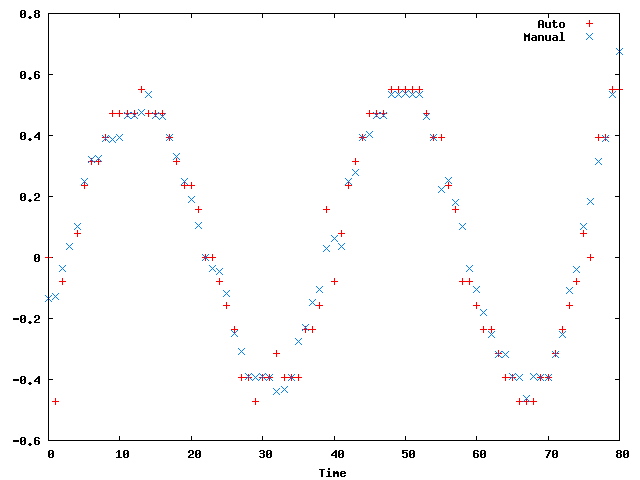
\includegraphics[width=\graphwidth]{../report/manualfitting/81-res10-leftthigh.png}}
        \quad
        \subfloat[Right thigh]{\label{ManualFit81:res10:RightThigh}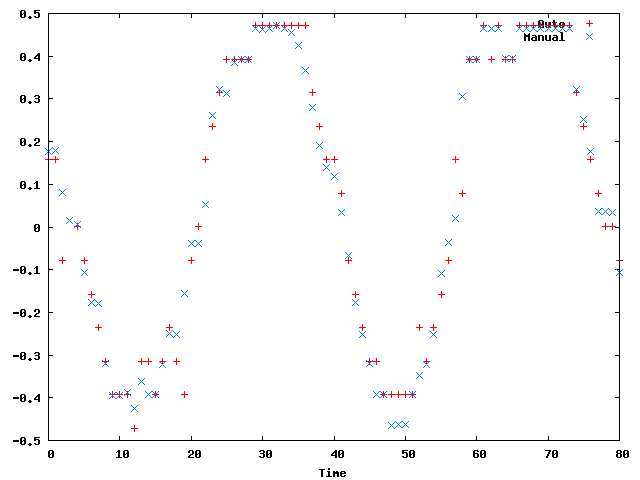
\includegraphics[width=\graphwidth]{../report/manualfitting/81-res10-rightthigh.png}}
        \
        \subfloat[Left lower leg]{\label{ManualFit81:res10:LeftLower}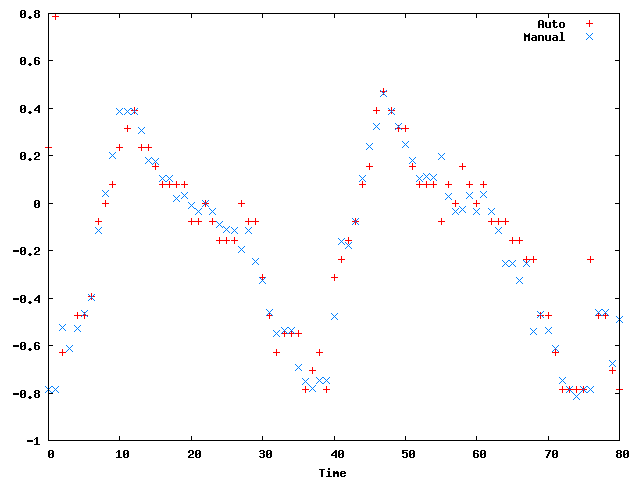
\includegraphics[width=\graphwidth]{../report/manualfitting/81-res10-leftlower.png}}
        \quad
        \subfloat[Right lower leg]{\label{ManualFit81:res10:RightLower}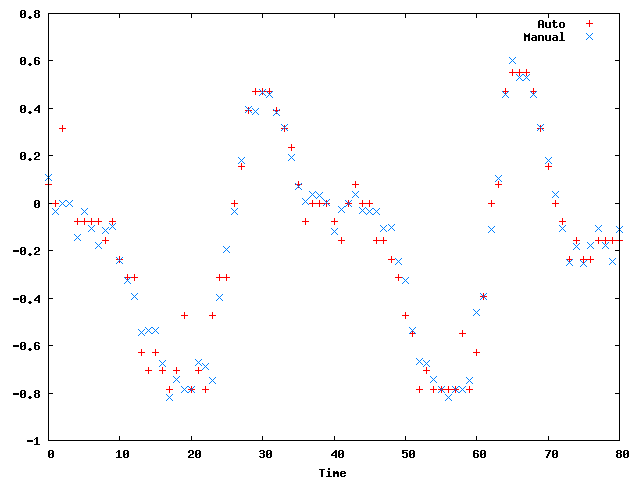
\includegraphics[width=\graphwidth]{../report/manualfitting/81-res10-rightlower.png}}

        \caption{Fitting error for Sample 81 using the low fixed resolution search.}
        \label{ManualFit81:res10}
\end{figure}

The overall low error rate for the modelfitting is encouraging.
As is to be expected, the lower resolution search is not quite as accurate as the high resolution search.
The multi-resolution search seems to perform even better, as its second pass has twice the equivalent resolution of the high fixed resolution search.

\clearpage
The sample data used to test the algorithms contains 10 different subjects.
Four recordings of each subject were taken, giving a total of 40 samples.
Two of the four samples from each subject were manually classified and entered into a database for use as a training set,
while the remaining two samples (labelled \emph{a} and \emph{b}) were put through automatic classification.

The success rate of the system was determined by how many of the ``unknown'' samples \emph{a} and \emph{b} it was able to match to the correct class in the training set.
In the tables below (\ref{ClassificationResults} and \ref{ClassificationResults2}) the numbers in each cell represent how close the algorithm came to correctly identifying the subject.
A value of 3 would indicate that there were 3 other classes that were a better match than the correct one,
while a value of 0 would represent a correct classification.

\bigskip
From Table \ref{ClassificationResults2} we can see that there is one winning combination in terms of correct classification rates.
This combination is summarised in Table \ref{ConclusionTable}.

\begin{table}[hb]
	\centering
	\begin{tabular}{r|l}
		Search resolution & res$_\theta$ = 21, res$_\alpha$ = 11 \\
		Multiresolution search? & No \\
		Parameters to include in the DFT & Both thigh $\theta$ values\\
		Number of DFT components to use & All \\
		Additional classifiers & Subject's height \\
		Normalise for mean? & Yes \\
		Normalise for variance? & No \\
		Distance measure & Euclidean distance in complex plane
	\end{tabular}
	\caption{Summary of the winning algorithm.}
	\label{ConclusionTable}
\end{table}

Our best algorithm gives a 90\% success rate when applied to our dataset.
The two samples that were classified incorrectly in this test (4a and 4b) were actually very close to receiving the correct classification - with only one or two other samples in between them and a sample of the correct class.

Previous research into gait recognition has typically produced algorithms that have success rates between 90\% and 100\%.
From this we can conclude that our results in 3D are at least as good as those in previous works.

\begin{landscape}
	\begin{table}[p]
		\centering
		\begin{tabular}{|l|c@{ }c|c@{ }c|c@{ }c|c@{ }c|c@{ }c|c@{ }c|c@{ }c|c@{ }c|c@{ }c|c@{ }c|c|}
			\hline
			& \multicolumn{20}{|c|}{Sample} & Success rate \\
			& 1a & 1b & 2a & 2b & 3a & 3b & 4a & 4b & 5a & 5b & 6a & 6b & 7a & 7b & 8a & 8b & 9a & 9b & 10a & 10b & \\
			
			\hline
			Magnitude                  & 1 & 2 & 1 & 0 & 0 & 1 & 6 & 11 & 4 & 0 & 3 & 0 & 0 & 2 & 0 & 0 & 1 & 2 & 2 & 0 & 40\% \\
			Phase-mag                  & 0 & 2 & 0 & 6 & 0 & 1 & 12 & 10 & 3 & 3 & 0 & 4 & 1 & 0 & 0 & 2 & 10 & 16 & 1 & 5 & 30\% \\
			Polar dist                 & 0 & 3 & 0 & 0 & 0 & 0 & 0 & 11 & 0 & 3 & 2 & 0 & 0 & 0 & 0 & 0 & 7 & 0 & 0 & 16 & 70\% \\
			Eucl dist                  & 0 & 3 & 0 & 0 & 0 & 0 & 0 & 11 & 0 & 3 & 2 & 0 & 0 & 0 & 0 & 0 & 7 & 0 & 0 & 16 & 70\% \\
			
			\hline
			Mag excl first             & 2 & 1 & 1 & 6 & 1 & 1 & 0 & 2 & 14 & 2 & 3 & 0 & 1 & 8 & 0 & 7 & 1 & 2 & 4 & 1 & 15\% \\
			Phase-mag excl first       & 0 & 2 & 0 & 6 & 0 & 1 & 12 & 12 & 3 & 3 & 0 & 2 & 1 & 0 & 0 & 2 & 10 & 2 & 1 & 15 & 30\% \\
			Polar dist excl first      & 0 & 2 & 0 & 2 & 0 & 0 & 0 & 11 & 0 & 5 & 3 & 0 & 0 & 0 & 0 & 2 & 9 & 0 & 2 & 16 & 55\% \\
			Eucl dist excl first       & 0 & 2 & 0 & 2 & 0 & 0 & 0 & 11 & 0 & 5 & 3 & 0 & 0 & 0 & 0 & 2 & 9 & 0 & 2 & 16 & 55\% \\
			
			\hline
			Eucl dist norm             & 0 & 2 & 0 & 0 & 0 & 0 & 0 & 11 & 0 & 0 & 4 & 0 & 0 & 0 & 0 & 0 & 7 & 0 & 0 & 16 & 75\% \\
			
			\hline
		\end{tabular}
		\caption{Comparison of different implementations of the distanceTo() function.}
		\label{ClassificationResults}
	\end{table}
	
	\begin{table}[p]
		\centering
		\begin{tabular}{|l|c@{ }c|c@{ }c|c@{ }c|c@{ }c|c@{ }c|c@{ }c|c@{ }c|c@{ }c|c@{ }c|c@{ }c|c|}
			\hline
			& \multicolumn{20}{|c|}{Sample} & Success rate \\
			& 1a & 1b & 2a & 2b & 3a & 3b & 4a & 4b & 5a & 5b & 6a & 6b & 7a & 7b & 8a & 8b & 9a & 9b & 10a & 10b & \\
			
			\hline
			\multicolumn{22}{|l|}{\textbf{Using both thigh $\theta$ values.}} \\
			Low res search             & 0 & 0 & 0 & 0 & 0 & 0 & 1 & 4 & 0 & 0 & 1 & 0 & 0 & 0 & 0 & 0 & 0 & 0 & 0 & 18 & 80\% \\
			High res search            & 0 & 1 & 0 & 0 & 0 & 0 & 1 & 5 & 0 & 1 & 2 & 0 & 0 & 0 & 0 & 0 & 8 & 0 & 0 & 18 & 65\% \\
			Multi res search           & 0 & 1 & 0 & 0 & 0 & 0 & 2 & 2 & 0 & 1 & 2 & 0 & 0 & 0 & 0 & 0 & 1 & 0 & 1 & 18 & 60\% \\
			
			\hline
			\multicolumn{22}{|l|}{\textbf{Using both lower leg $\theta$ values.}} \\
			Low res search             & 0 & 0 & 0 & 2 & 0 & 1 & 2 & 0 & 1 & 5 & 0 & 1 & 0 & 0 & 0 & 4 & 0 & 0 & 0 & 18 & 60\% \\
			High res search            & 0 & 0 & 0 & 0 & 0 & 0 & 2 & 2 & 1 & 5 & 1 & 2 & 0 & 0 & 1 & 3 & 4 & 1 & 0 & 17 & 45\% \\
			Multi res search           & 0 & 2 & 0 & 0 & 0 & 0 & 4 & 4 & 2 & 5 & 1 & 1 & 0 & 0 & 0 & 0 & 4 & 2 & 0 & 17 & 50\% \\
			
			\hline
			\multicolumn{22}{|l|}{\textbf{Using both thigh and lower leg $\theta$ values.}} \\
			Low res search             & 0 & 0 & 0 & 1 & 0 & 0 & 1 & 2 & 0 & 3 & 0 & 1 & 0 & 0 & 0 & 0 & 3 & 0 & 0 & 18 & 65\% \\
			High res search            & 0 & 0 & 0 & 0 & 0 & 0 & 1 & 2 & 0 & 4 & 2 & 1 & 0 & 0 & 0 & 0 & 4 & 0 & 0 & 18 & 65\% \\
			Multi res search           & 0 & 1 & 0 & 0 & 0 & 0 & 3 & 3 & 0 & 4 & 0 & 0 & 0 & 0 & 0 & 0 & 3 & 1 & 0 & 18 & 65\% \\
			
			\hline
			\multicolumn{22}{|l|}{\textbf{Including the subject's height as an additional classifier}} \\
			Low res search             & 0 & 0 & 0 & 0 & 0 & 0 & 2 & 1 & 0 & 0 & 0 & 0 & 0 & 0 & 0 & 0 & 0 & 0 & 0 & 0 & 90\% \\
			
			\hline
		\end{tabular}
		\caption{Comparison of different modelfitting algorithms and parameters.
			These tests all use the mean-normalising Euclidean distance function from the previous page.}
		\label{ClassificationResults2}
	\end{table}
\end{landscape}

\newpage
\bibliography{../../bibtex}

\end{document}
